\chapter{Conclusion}

\begin{figure}[h!]
	\caption{Application Main Page}
	\label{image:dashboard}
	\centering
	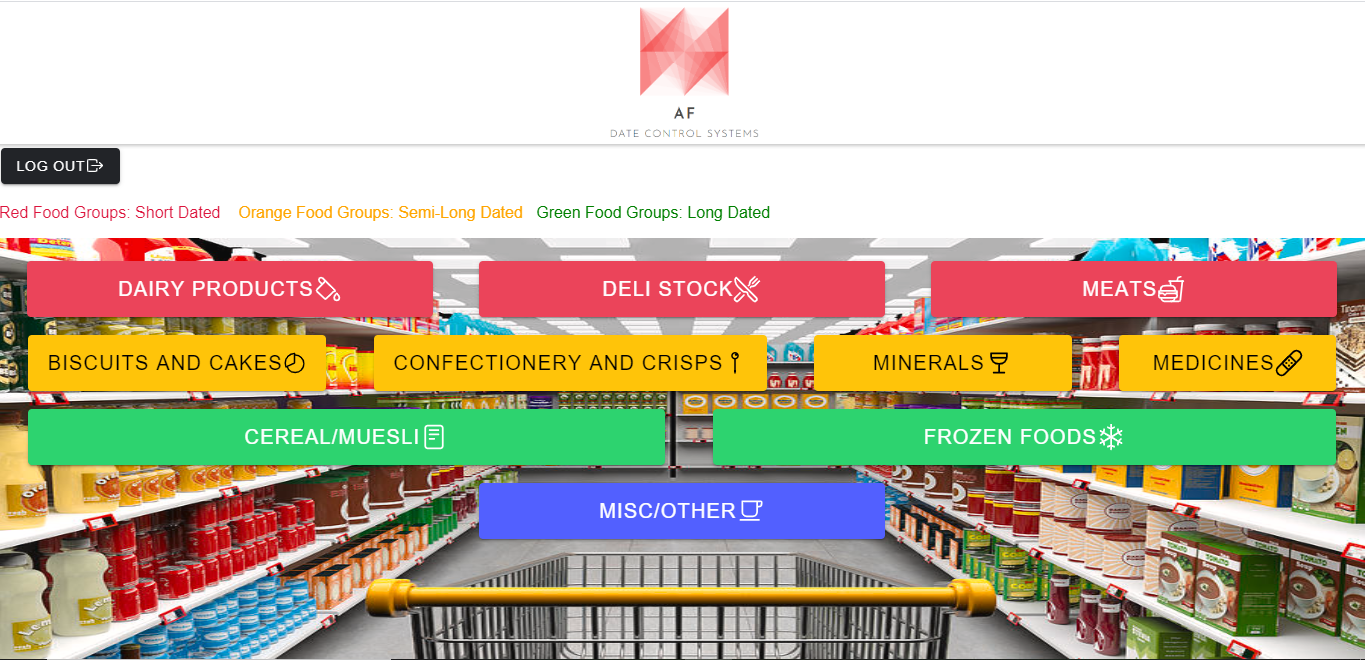
\includegraphics[width=1\textwidth]{images/dashboard.PNG}
\end{figure}

To conclude, from the outset the overall rationale and goals set out were to make an application that i felt along with second opinions from those i work with to create and develop a software application intended to tackle an exiting issue within the workplace that being date checking sufficiency, save staff members time in their already busy routine and save the shop money in terms of getting to a product in time to take action and for tactical ordering in the future. Not only does this application target supermarkets in terms of implementation, but also targets companies such as CBE mentioned throughout this dissertation. 
\newline
\newpage
Food wastage and Stock Control is proven to be an issue globally according to my research. The purpose of this application is to help suppress this issue. With the measures currently in place of date checking physically with the human eye, i feel this is not a sufficiently sustainable method as the human eye cannot see everything. This application shows the products that are close to their sell by dates or past them. This allows for staff members to log in to this application and identify the exact products that are close or past their sell by date, eliminating the danger of a customer potentially buying and consuming an out of date food item. This application proves to also reduce that potentially dangerous risk as well. Not all customers look at the best before date, imagine an elderly customer picks this item up and consumes it without knowing, this can be very harmful. I strongly believe this application intercepts this scenario. 
\newline

Not every single objective i wanted to meet were met in the development of this application. However i feel the main objectives set out from the start were met and for that i am very satisfied with the outcome which i believe to be successful. It is providing a helpful service to a place i have worked part time in for five years. The flexibility and versatility of this application is very beneficial. Not only can it be for its intended purpose but it can also aid the weekly reports side of things such as staff HACCP forms where the staff member records items taken off the shelf due to damage or in this case their sell by date. The application can easily be altered this way due to the very flexible Ionic framework and firebase cloud storage being able to tweak certain aspects to match the need at the time. 
\newline

I believe using Ionic Firebase was the right technology option not only for me for development but the overall look and functionality of the application. The application needed to be easy for the staff member to use and understand. It also needed to be aesthetically pleasing to look at but at the same time not look too complex for usage. I believe in this case i have produced this, as you can see in the dashboard of the application screenshot above the food groups divided into color coded sections, Red for short dated products for example. 
\newline

\subsection{Outcomes of the Project}
- Gained more knowledge and understanding about the technologies used from the start to finish of this projects development and delivery. I learned a lot more about the Ionic Framework in terms of its functionality and capabilities. My understanding of the Firebase Cloud Database has been enhanced as a result of producing this project. For example making my application a Firebase hosted website which then gave me a sense of accomplishment after typing in the URL of my application and it showing up rather than doing an ionic serve which runs the application on the local host. Not to mention enhancing my skill in usage of GitHub looking at insights and highlighting issues, Visual Studio Code in showing me if i need to commit changes to GitHub or install a certain package required for the application functionality and Overleaf LaTeX newly learnt framework in which my experience using it in other projects helped me in writing this dissertation.
\newline

- I feel i have improved in my weekly goals and objectives delivery with the weekly meetings i had with my supervisor who was a great help throughout the development of this project in listening to me as a student and giving valuable advice for certain things. My supervisor provided me with feedback every week in which i would always take on board be it positive or negative. 
\newline

- Another outcome being that i have produced an application to help with an existing issue linked to life outside the college environment. That of course being in the workplace. The thought of producing an application to help save staff members time, gave me enough encouragement to produce this application to make for a happier place to work for all.
\newline

- Minor outcomes such as conducting surveys and application tests was also an important outcome from the project. Conducting a survey and receiving feedback is highly important in the development of an application as it gives you a rough indication of if an application is indeed necessary. Also conducting an application test to show the users or viewers what works and what doesn't and a small step by step snippet of how to use each function. I have done application testing for past projects also. These were done specifically to give the viewer and user more insight into the project/application.

- A sense of self accomplishment was one of if not the main outcome of doing this project. Seeing this application in action and a sense of "a proud moment" when demonstrating this application to my friends, family and work colleagues and saying i made that. This is my favourite outcome in which i will not forget.   
\newline
\subsection{Personal}
Overall as a final year student i am extremely satisfied with what i have developed for my final year project. When finishing and presenting i get this unique feeling of self accomplishment. I have brought my college experience and my work experience together and created an application. AF-Date-Control-Systems an application that was created to solve an issue within retail relating to date checking and food wastage. That is what i myself have created, a prototype application potentially for use in the shop i work in or even beyond. 
\newpage
This project may also aid me in potential employment in the future with CBE in which i have contacted via email but understandably during these unusual times i am yet to hear back from them, however i remain optimistic and maybe i will be allowed to demonstrate my application to CBE or even meet with someone from CBE to explain how this application can be implemented into their systems and how it can save them time and money providing this new and effective service to their customers. I enjoyed every moment of doing this project as it links to life outside college in which i enjoy to discuss my part time job with others and use my knowledge gained from GMIT for the past four years to show what i have learned and remembering this project for life. Also due to the fact that this has not yet been implemented into retail as of yet, i get the sense of a "first" to come up with this idea. I am excited to get the feedback from those who may have the capabilities to implement this such as CBE to see if this can be possible and presenting an idea to them before employment would benefit me in the long run. I am pleased to say this project can go many places if implemented and explained correctly, and the fact i have done this is most satisfying to read and hear. Fin.

